% Chapter 7

\chapter{Resultados} % Main chapter title

\label{Chapter7} % Change X to a consecutive number; for referencing this chapter elsewhere, use \ref{ChapterX}

El objetivo de este capítulo fue el de brindar resultados para distintos escenarios de interés, con el fin de dar comparaciones analíticas con base en la variación de los parámetros de entrada del simulador.

%----------------------------------------------------------------------------------------
%	SECTION 
%----------------------------------------------------------------------------------------

\section{Escenario I} % Simulación con un solo un TTI - FER
\subsection{Descripción del escenario}
Este escenario se concentró en\dots

\subsection{Parámetros de entrada}


\subsection{Resultados obtenidos}

\begin{figure}[th]
    \centering
    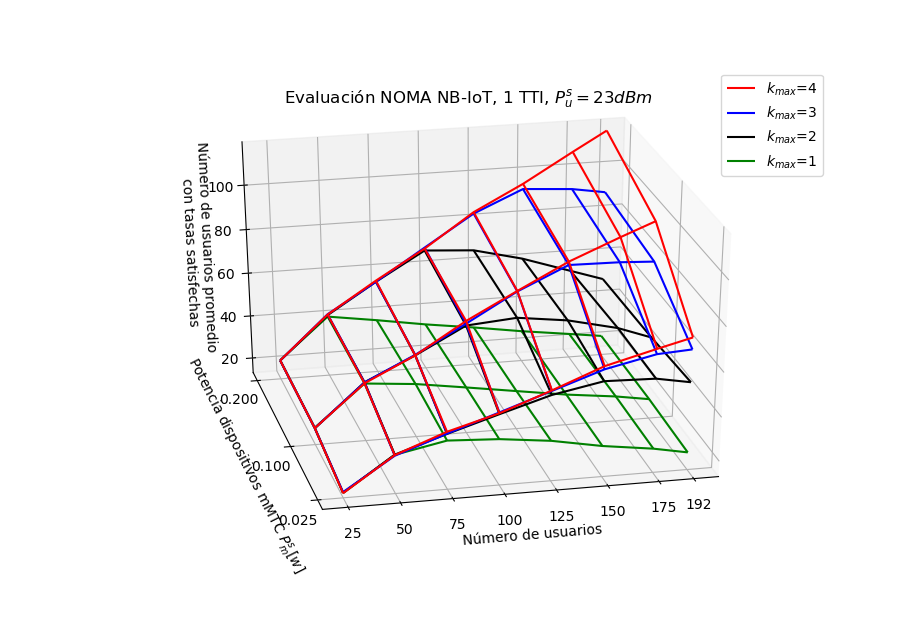
\includegraphics[scale=.7]{Figures/ResultadosNOMA/NOMA_evaluacion_K_Pm_Variable_3D.png}
    \decoRule
    \caption[]{}
    \label{fig:}
\end{figure}

\begin{figure}[th]
    \centering
    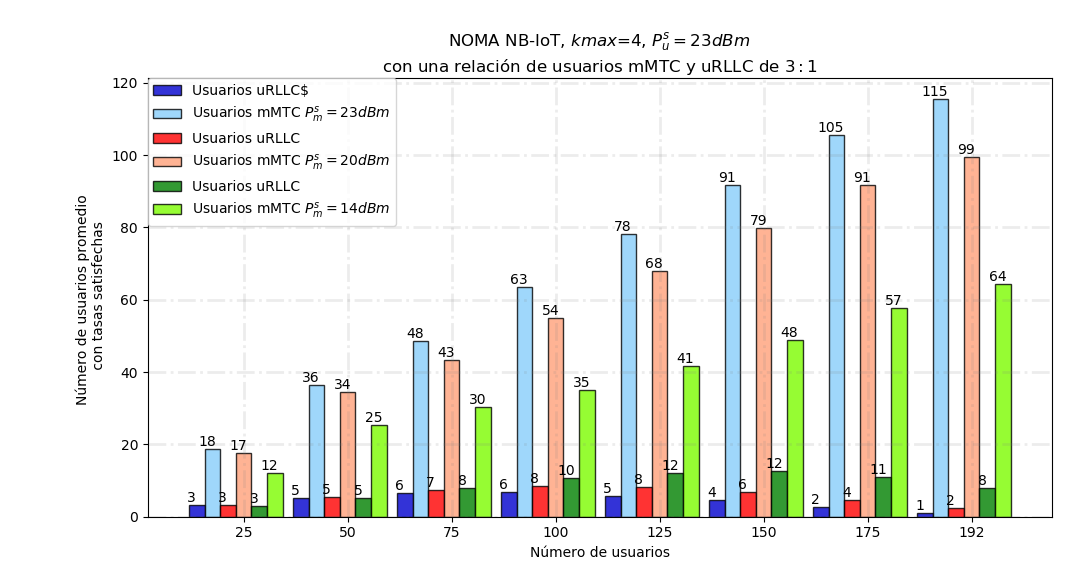
\includegraphics[scale=.6]{Figures/ResultadosNOMA/Kmax4_DiferentesPM.png}
    \decoRule
    \caption[]{}
    \label{fig:}
\end{figure}

\begin{figure}[th]
    \centering
    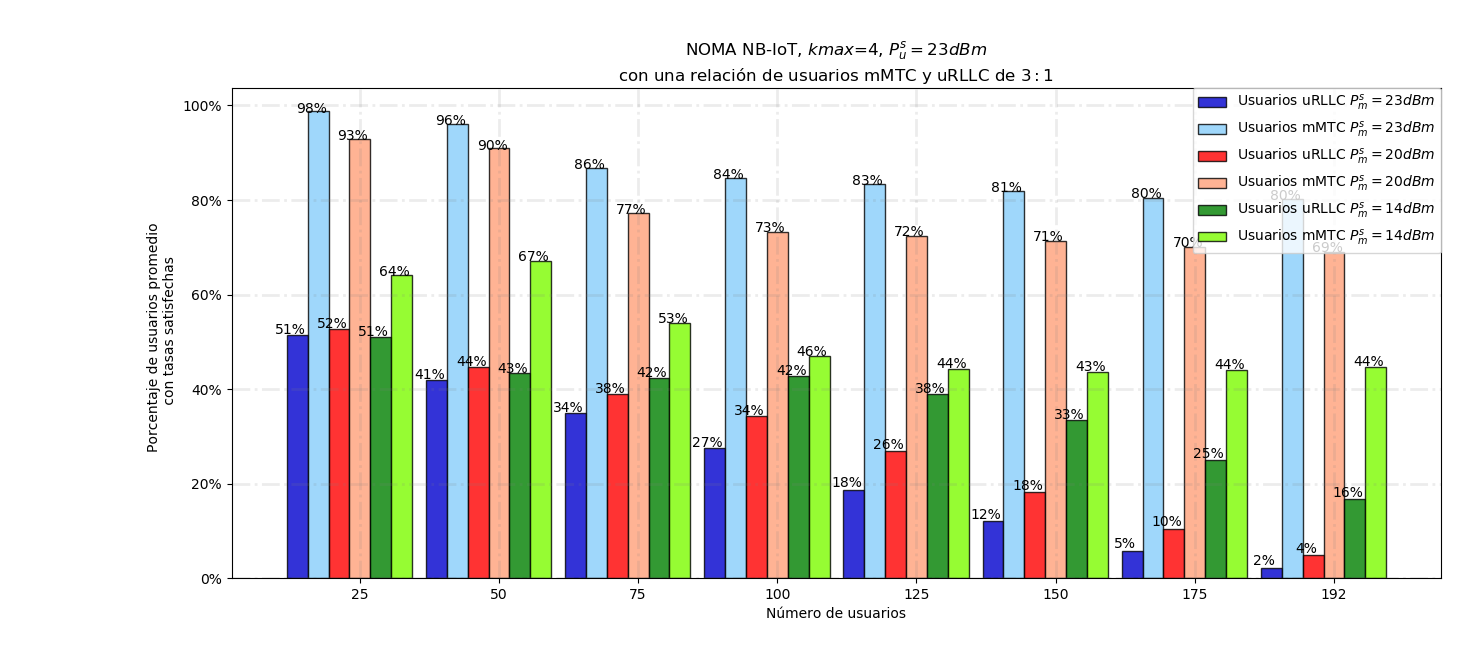
\includegraphics[scale=.4]{Figures/ResultadosNOMA/Kmax4_DiferentesPM_Porcentual.png}
    \decoRule
    \caption[]{}
    \label{fig:}
\end{figure}

\begin{figure}[th]
    \centering
    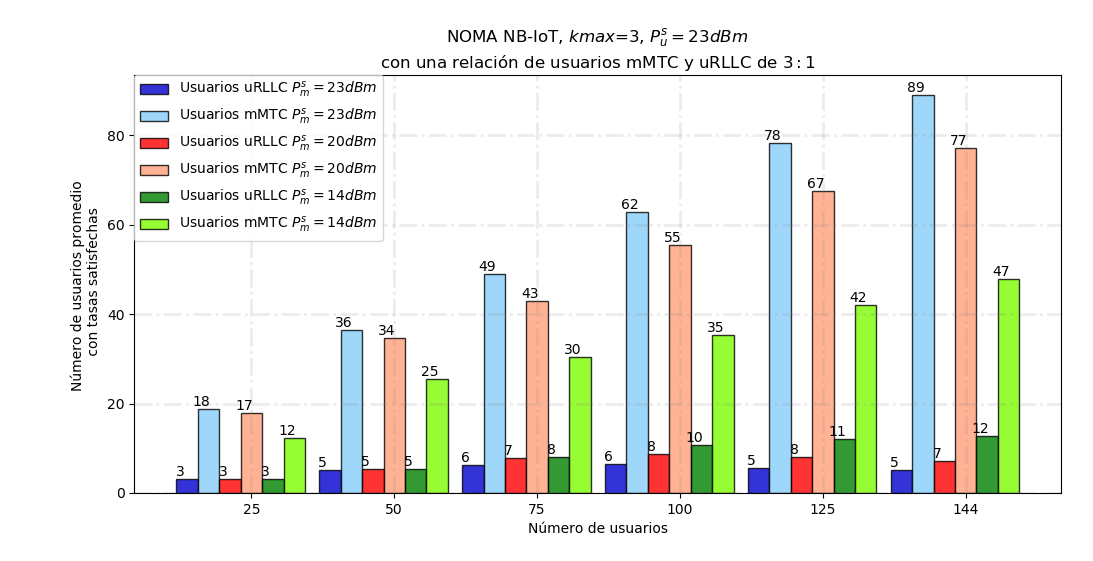
\includegraphics[scale=.6]{Figures/ResultadosNOMA/Kmax3_DiferentesPM.png}
    \decoRule
    \caption[]{}
    \label{fig:}
\end{figure}

\begin{figure}[th]
    \centering
    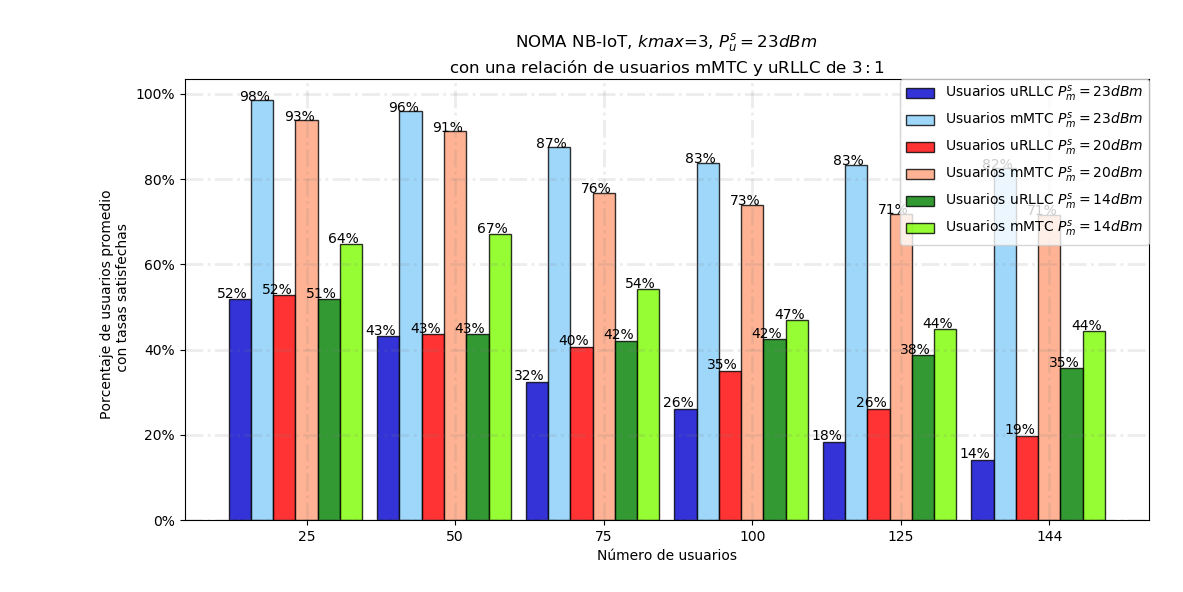
\includegraphics[scale=.6]{Figures/ResultadosNOMA/Kmax3_DiferentesPM_Porcentual.png}
    \decoRule
    \caption[]{}
    \label{fig:}
\end{figure}

\begin{figure}[th]
    \centering
    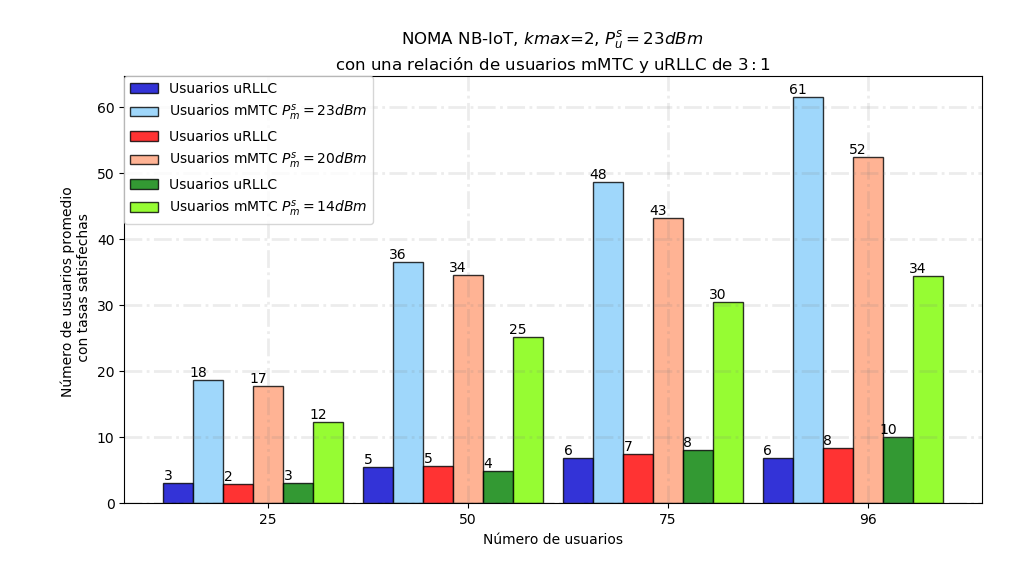
\includegraphics[scale=.5]{Figures/ResultadosNOMA/Kmax2_DiferentesPM.png}
    \decoRule
    \caption[]{}
    \label{fig:}
\end{figure}

\begin{figure}[th]
    \centering
    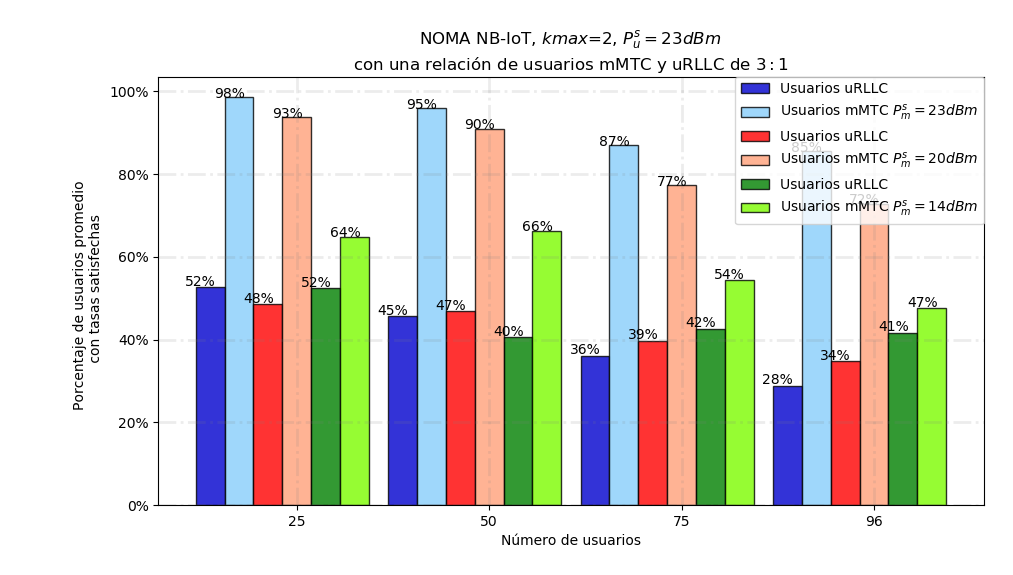
\includegraphics[scale=.6]{Figures/ResultadosNOMA/Kmax2_DiferentesPM_Porcentual.png}
    \decoRule
    \caption[]{}
    \label{fig:}
\end{figure}


\begin{figure}
    \centering
    \begin{minipage}{.45\linewidth}
      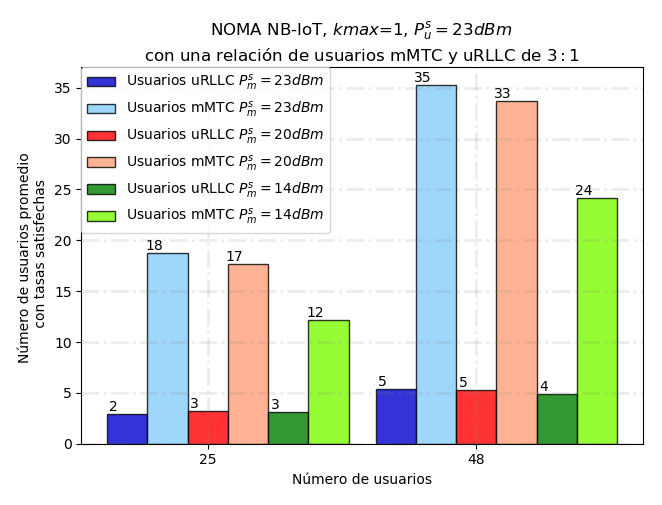
\includegraphics[width=\linewidth]{Figures/ResultadosNOMA/Kmax1_DiferentesPM.png}
      \captionof{figure}{}
      \label{fig:img1}
    \end{minipage}
    \hspace{.0\linewidth}
    \begin{minipage}{.45\linewidth}
      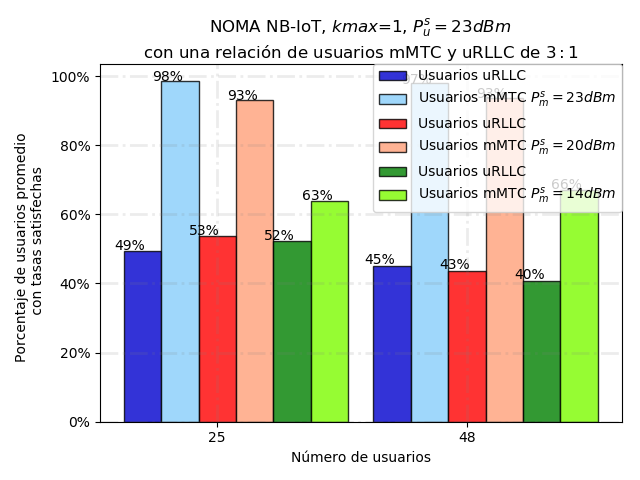
\includegraphics[width=\linewidth]{Figures/ResultadosNOMA/Kmax1_DiferentesPM_Porcentual.png}
      \captionof{figure}{}
      \label{fig:img2}
    \end{minipage}
\end{figure}


%----------------------------------------------------------------------------------------
%	SECTION 
%----------------------------------------------------------------------------------------

\section{Escenario II} % Simulación completa con tráfico - ROLANDO
\subsection{Descripción del escenario}
\subsection{Parámetros de entrada}
\subsection{Resultados obtenidos}

